\section{Introduction}
\label{sec:intro}

Pretrained Vision Transformers \citep{dosovitskiy2021vit,steiner2022augreg} are usually adapted to a new task instead of being trained from scratch, either by fine-tuning all weights or by training a small number of added parameters \citep{houlsby2019adapter,hu2022lora,chen2022adaptformer}.
In this project we adapt ViT-B/16 to a fine-grained dataset with 10,000 classes whose names are hidden.
There are 45 training images per class (450,000 in total); the labels of the validation set (50,000 images) and the test set (100,000 images) are hidden and scored on CodaBench.
Each training run may use 2 hours on 48\,GB of GPU memory, which is 1.2 hours on our 80\,GB A100.

\begin{figure}[b]
  \centering
  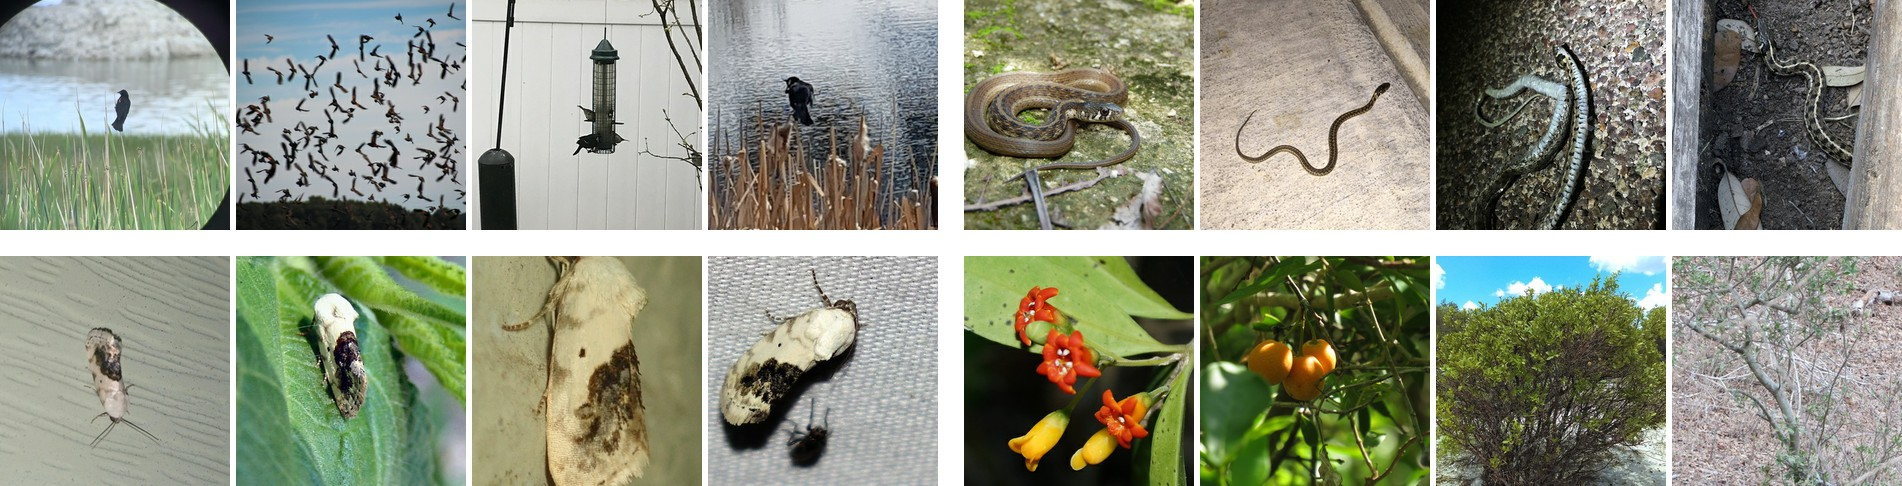
\includegraphics[width=\linewidth]{figures/data_examples_wide.jpg}
  \caption{\textbf{Training images of four of the 10,000 classes.} Each group of four is one class (a bird, a snake, a moth and a plant): one bird or a whole flock, a flower or a whole shrub. Each class has only 45 such images.}
  \label{fig:examples}
\end{figure}

\paragraph{Why this is hard.}
As \cref{fig:examples} shows, one class can look very different from image to image, while different classes in a fine-grained dataset can look alike, and each class has only 45 images.
A model can easily memorize such a small set, so a low training loss tells us little; every choice has to be judged on held-out images.
The new classifier head is also large: a $10{,}000 \times 768$ layer has 7.69M parameters, 9\% of the 85.8M-parameter backbone, and each of its rows is trained on only 43--45 images.
Finally, the budget is tight: one epoch of full fine-tuning takes about 7 minutes, so only about eight epochs fit into one run.

\paragraph{Our objectives.}
A high leaderboard score was not our only goal.
We wanted to answer three questions.
(1)~What limits accuracy when there are many classes but few images per class, and how can we fix it?
(2)~If we compare adaptation methods fairly, with one protocol and one budget, where do trainable parameters help most, and what does each method cost in memory and latency?
(3)~How should a fixed budget be split between epochs, training data and test-time computation?
We answered them with 26 runs, each changing one setting, and chose models on a local holdout split that matches the CodaBench validation score within 0.3 points.
Our contributions are:
\begin{itemize}[leftmargin=*,itemsep=1pt,topsep=2pt]
    \item \textbf{A better start for the head.} The linear-probe (LP) head used by LP-FT \citep{kumar2022lpft}, trained on frozen features of the training images, hurts in our task. Starting each class from its normalized mean feature (a prototype) instead adds 2.1--3.1 points for full fine-tuning, LoRA and AdaptFormer. A random-head control shows that the harm comes from fitting the head on the training images (\cref{sec:ablation-head}).
    \item \textbf{A fair comparison of seven adaptation methods.} Small changes in every block give much more accuracy per parameter than fine-tuning the top blocks: LoRA on 1.375\% of the backbone matches the last four blocks (33\%). Training memory depends on how far back the gradients go, not on how many parameters are trained (\cref{sec:compare}).
    \item \textbf{Final results with their full cost.} Our final models reach 76.22\% (full fine-tuning, $+$5.4 over the reference) and 71.90\% (LoRA, $+$3.6 over the reference LoRA) on the validation set, and 76.09\% and 71.67\% on the test set, within the budget (\cref{sec:main}).
    \item \textbf{The process, including failures.} We report the study round by round, with the ideas that failed (\cref{sec:process}), and find after the deadline that larger input images add 4.4 points (\cref{sec:post}).
\end{itemize}
